\section{Tài nguyên}
\subsection{Nguồn dữ liệu}
% hoang
Tập dữ liệu được sử dụng trong nghiên cứu này được lấy từ \underline{https://finance.yahoo.com/}, một nền tảng tài chính uy tín được biết đến với thông tin thị trường toàn diện và cập nhật. Tập dữ liệu bao gồm dữ liệu giá cổ phiếu của ba ngân hàng nổi tiếng tại Việt Nam: Ngân hàng Đầu tư và Phát triển Việt Nam (BIDV), Ngân hàng Thương mại Cổ phần Xuất Nhập Khẩu Việt Nam (Eximbank) và Ngân hàng Thương mại Cổ phần Ngoại Thương Việt Nam (Vietcombank). Bằng cách tận dụng dữ liệu có sẵn trên nền tảng này, chúng tôi đảm bảo một nền tảng đáng tin cậy cho phân tích của mình. Tập dữ liệu bắt đầu từ ngày 1 tháng 3 năm 2019 đến ngày 1 tháng 3 năm 2024, cung cấp một phạm vi thời gian mạnh mẽ cho phân tích của chúng tôi. Mỗi mục trong tập dữ liệu bao gồm các chỉ số tài chính chính, bao gồm:
\begin{itemize}
\item \textbf{Date}: Ngày giao dịch.
\item \textbf{Open}: Giá cổ phiếu mở cửa vào đầu ngày giao dịch.
\item \textbf{High}: Giá cổ phiếu cao nhất ghi nhận được trong ngày giao dịch.
\item \textbf{Low}: Giá cổ phiếu thấp nhất ghi nhận được trong ngày giao dịch.
\item \textbf{Close}: Giá cổ phiếu đóng cửa vào một ngày nhất định.
\item \textbf{Adj Close}: Giá đóng cửa được điều chỉnh, bao gồm bất kỳ hành động doanh nghiệp nào như cổ tức hoặc chia cổ phiếu.
\item \textbf{Volume}: Khối lượng giao dịch, chỉ ra tổng số cổ phiếu được giao dịch vào một ngày cụ thể.
\end{itemize}
\subsection{Descriptive Statistics}
\begin{figure}[H]
    \centering
    \begin{minipage}{0.23\textwidth}
    \centering
    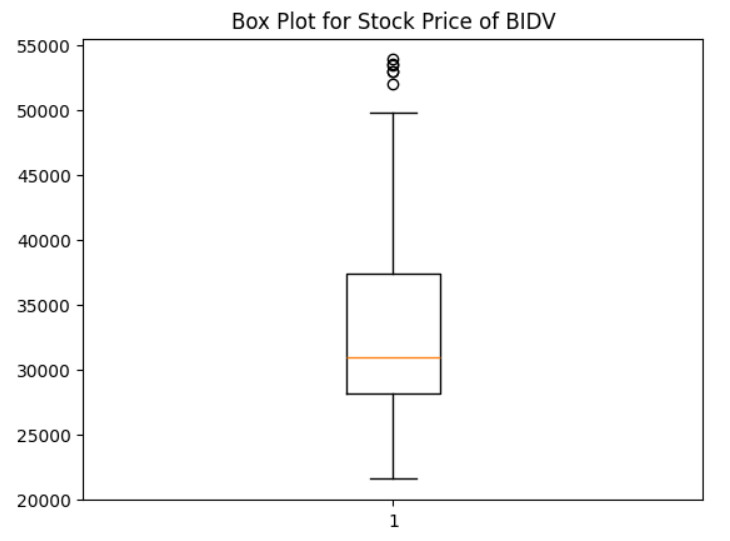
\includegraphics[width=1\textwidth]{resources/chapter-3/Boxplot_BIDV.jpg}
    \caption{BIDV stock price's boxplot}
    \label{fig:bidv_boxplot}
    \end{minipage}
    \hfill
    \begin{minipage}{0.23\textwidth}
    \centering
    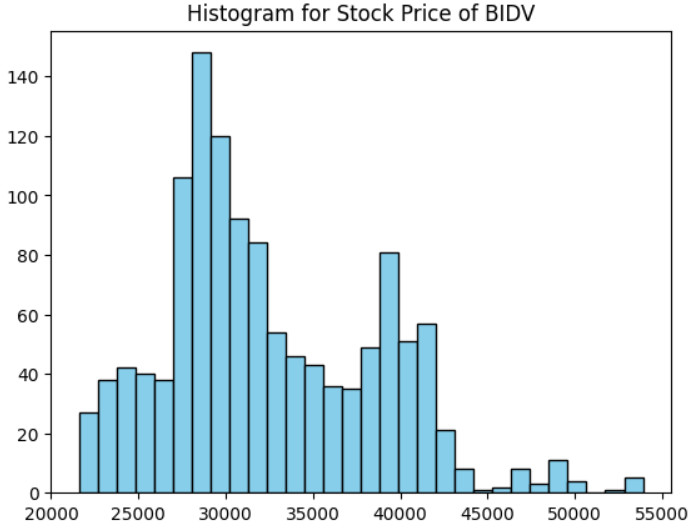
\includegraphics[width=1\textwidth]{resources/chapter-3/Histogram_BIDV.jpg}
    \caption{BIDV stock price's histogram}
    \label{fig:bidv_histogram}
    \end{minipage}
\end{figure}

\begin{figure}[H]
    \centering
    \begin{minipage}{0.23\textwidth}
    \centering
    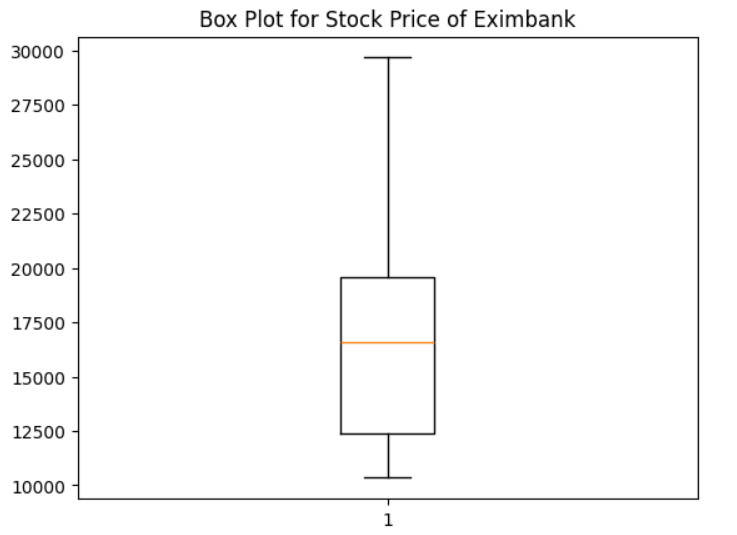
\includegraphics[width=1\textwidth]{resources/chapter-3/Boxplot_Eximbank.jpg}
    \caption{Eximbank stock price's boxplot}
    \label{fig:eximbank_boxplot}
    \end{minipage}
    \hfill
    \begin{minipage}{0.23\textwidth}
    \centering
    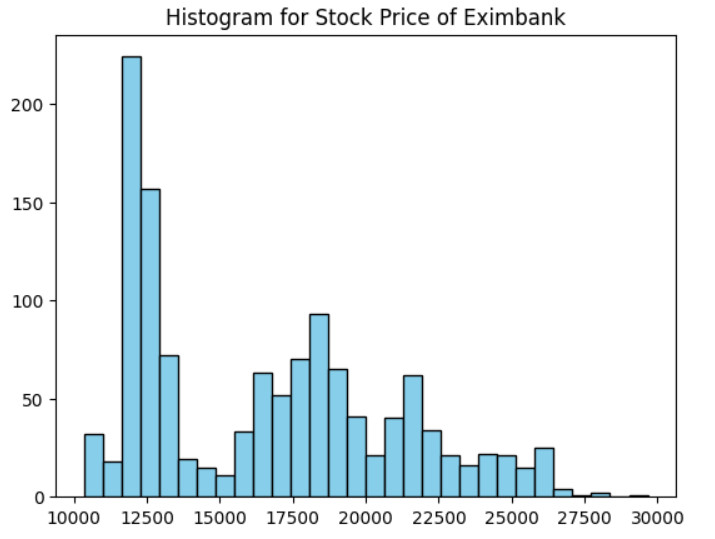
\includegraphics[width=1\textwidth]{resources/chapter-3/Histogram_Eximbank.jpg}
    \caption{Eximbank stock price's histogram}
    \label{fig:eximbank_histogram}
    \end{minipage}
\end{figure}

\begin{figure}[H]
    \centering
    \begin{minipage}{0.23\textwidth}
    \centering
    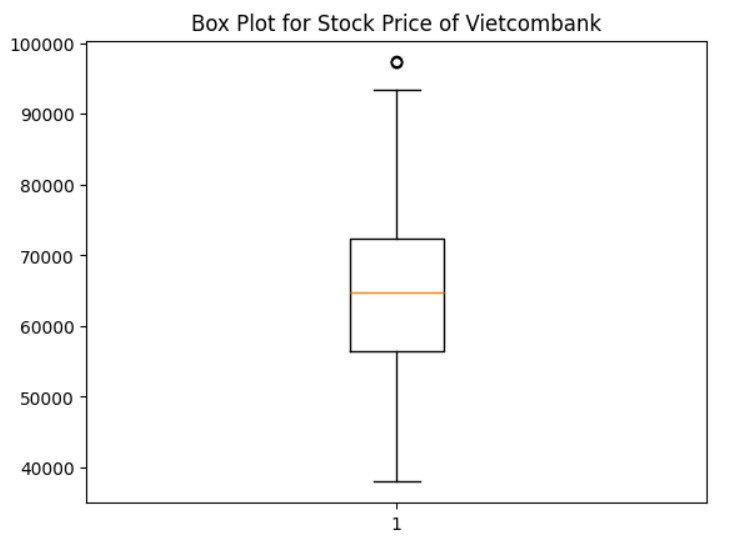
\includegraphics[width=1\textwidth]{resources/chapter-3/Boxplot_Vietcombank.jpg}
    \caption{VCB stock price's boxplot}
    \label{fig:vcb_boxplot}
    \end{minipage}
    \hfill
    \begin{minipage}{0.23\textwidth}
    \centering
    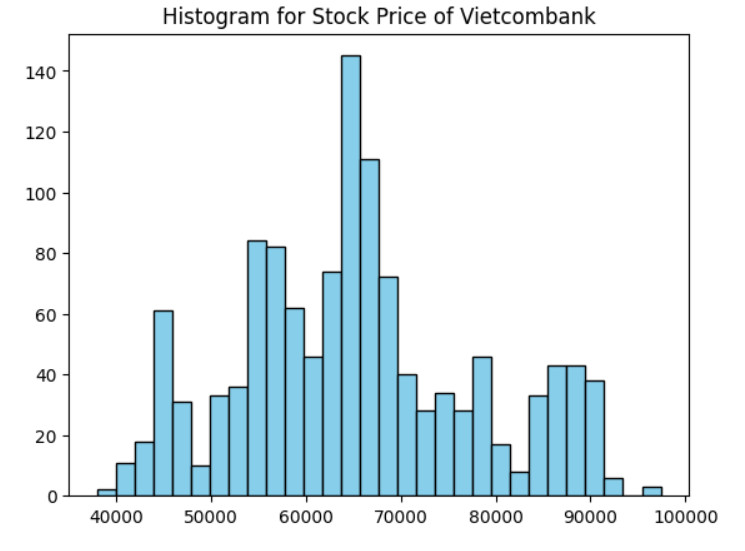
\includegraphics[width=1\textwidth]{resources/chapter-3/Histogram_Vietcombank.jpg}
    \caption{VCB stock price's histogram}
    \label{fig:vcb_histogram}
    \end{minipage}
\end{figure}

\subsection{Công cụ}
Trong nghiên cứu của chúng tôi, chúng tôi đã sử dụng các công cụ phân tích thống kê khác nhau trong Python để hiểu rõ hơn dữ liệu và đưa ra những kết luận ý nghĩa. Các công cụ này, bao gồm numpy, pandas, sklearn và matplotlib.pyplot, đã giúp chúng tôi khám phá ra những phát hiện đáng chú ý. Để biết kết quả chi tiết, vui lòng xem bảng mô tả và biểu đồ được cung cấp.
% end hoang

% long
\subsection{Tỷ lệ phân chia tập dữ liệu}
Nội dung.

\subsection{Các chỉ số đánh giá mô hình}
Nội dung.
% end long